データを符号化して保存できたら、これを相手に送ったり、あるいは受け取ったりする。これがまさしく通信そのものである。最も単純な方法は物理的に媒体をやり取りする―\textbf{スニーカーネット}\index{すにーかーねっと@スニーカーネット}―だが、空間や時間の制限故に常にこれが最適とは限らない\footnote{ここでは「最適とは限らない」と書いたが、最適な場合も勿論ある。データとしてやり取りできないもの:例えば物理的なプレゼントなどは言うまでもないが、データにおいてもスニーカーネットが最善となる例は少なくない。用意されている通信路に対して送るデータがあまりに膨大な場合は宅配便などで記憶媒体を直接送付するほうが良い場合も多い。「新幹線に目一杯HDD積んで走らせるのが最も伝送速度が速い方法だ」などというジョークもあるが、電気的に記録されたデータのやり取りとしてスニーカーネットは決して過去の遺物ではないのである。}。電気的にデータをやり取りできれば、ごく短時間で遠く離れた場所への通信も可能となる。電話・ラジオ・テレビなどがごく身近な例といえる。

電気的なデータのやり取りには電気的な接続が必要となる。先の例でも、電話やテレビはそれぞれ電話線・アンテナケーブルなどで電気的に繋がっており、ラジオは電波で電気的に繋がっている。本章ではこの「接続」について学んでいこう。

\section{伝送路に求められる性質}
電気通信においては、アナログデータをそのまま電圧変化などの電気的信号に変えて伝送するケースも考えられるが、多くの場合符号化したデータを伝送するデジタルデータ伝送となる。ここで用いられる符号は一般に2進符号である。これを送るために、どのような性質があれば望ましいだろうか。

電気的な信号をやり取りする場合、電圧変化が信号に対応する。このとき、元々流れている何らかの電気(直流のときもあれば交流のときもある)からの変化が信号に対応する。この変化が見やすいこと、つまり「どこから信号が始まるか」がわかりやすいということが通信には都合が良い。また、安全のために電圧変化によって遮断されてしまう場合(遮断特性)があるが、これに影響されがちな通信路・方式は不都合である。他にも、伝送時にいつも雑音が入るような伝送路では伝送が正しく行われないし、雑音や遮断の状況が見えないようでは運用しづらい。

これらをまとめると、次のような性質がある伝送路が望ましいと言えるだろう。

\begin{itembox}[l]{伝送路に求められる性質}
\begin{itemize}
\item 情報の始点終点の検出などが容易である
\item 遮断特性の影響を受けにくい
\item 雑音に強い
\item 回線が容易に監視できる
\end{itemize}
\end{itembox}

\subsection{雑音}
先に\textbf{雑音}\index{ざつおん@雑音}という言葉を用いた。雑音というと例えば録音したものに余計な話し声が入っている場合などを想像するだろうが、通信においても同様である。混入することで通信の妨げとなるような伝送したい信号以外の(=希望しない)不規則性信号を雑音というのである。雑音に強い特性というのは\textbf{信号対雑音比}\index{しんごうたいざつおんひ@信号対雑音比}(S/N比\index{S/Nひ@S/N比|see{信号対雑音比}}Signal-to-noise ratio)が小さいということに対応する。S/N比とは読んで字のごとく、信号に対しどの割合で雑音が入るかという雑音の指標である。勿論、これが0に近いほうがより良い回線である。

以下、雑音の例を見てみよう。

\subsubsection{白色雑音・有色雑音}
電気的な理由などで全ての周波数帯に等しく雑音が出る場合、これを\textbf{白色雑音}\index{はくしょくざつおん@白色雑音}という。対して、周波数帯に偏りがある場合は\textbf{有色雑音}\index{ゆうしょくざつおん@有色雑音}と呼ばれる。

\subsubsection{インパルス性雑音}
自動車のエンジンの点火系統などから発生することのある、瞬間的かつ大きな雑音のことを\textbf{インパルス性雑音}\index{いんぱるすせいざつおん@インパルス性雑音}と呼ぶ。電気の突然の遮断などによって発生することもある。先に書いた「遮断特性の影響を受けにくい」というのは、インパルス性雑音が発生しにくいという条件の一つである。

\subsubsection{干渉信号・漏話}
通信路というのは、普通複数人で共用していたり、隣あっていたりするものである。このとき、別の通信で使用している信号が漏れてきて混入してしまうことがある。これを\textbf{干渉信号}\index{かんしょうしんごう@干渉信号}と呼ぶ。無線通信で近隣から同一周波数の電波があった場合などの干渉が代表的な例である。また、複数の電気線が束ねられている場合などは信号が別ケーブルから漏れ聞こえてくることもある(漏話・クロストーク)。

\subsubsection{受信信号の歪み}
通信時の中継器などでは、電気信号を増幅させるものが含まれることがある。このとき、非線形な入力特性をもつ増幅回路、つまり増幅後の電圧と増幅前の電圧の比が一定値にならないような増幅回路が存在すると、受信信号を歪めてしまうことがある。特に(あとで説明する)帯域伝送において、入力信号の周波数の和・差になるような別周波数の信号が生成されてしまう場合などが挙げられる。

\subsection{通信の品質}
通信路を実際に用意する場合、先に書いたような特性が水準以上であることが求められる。これらを評価する技術的な指標として、接続基準・安定基準・伝送基準の3つの基準が定められている。

\subsubsection{接続基準}
\textbf{接続基準}\index{せつぞくきじゅん@接続基準}とは、サービス要求がどの程度迅速・確実に相手に接続されるまでの時間の基準である。例えば、電話であればダイヤルしてから最大どの程度の時間で相手に接続されるべきかなどを示した基準である。問い合わせなどでの「何日以内で返信」などというのも広い意味では接続基準と言える。通常は時間の単位で評価する。ネットワークではタイムアウト値(=接続がこの値以上ないと通信が遮断されているとみなす)がこの基準に関係した値である。

接続基準は短いほど品質が良いが、短いということは通信相手側の反応を上げるということでもあるので当然システム側へ負荷がかかる。このため、システム負荷として許容可能な範囲で短く設定するのが基本となる。

\subsubsection{安定基準}
\textbf{安定基準}\index{あんていきじゅん@安定基準}とは、サービスそのものを提供できるかどうかの信頼性に関する基準である。通常、稼働率または不稼働率が使われる。稼働率とは「稼働する平均(見込み)時間」を「稼働が希望される期間」で割った比率で、これが高いほど希望されているうちでのサービスそのものの提供時間が長いということである。回線の場合、サービスとは通信であり、その回線を用いて通信できる時間の割合を示していると言って良い。

注警報の伝達や緊急通報など、「止めることが許されない」サービスにおいては、稼働率を高めるために予備設備を準備するなどの冗長化を行わなければならない。一方、人命などに関わるわけではないネットゲームなどでは、随時のメンテナンスなどでサービスを停止することも許され、稼働率はプレイヤーが飽きない程度であれば問題ない。このように、安定基準はシステムの特性に応じて特に水準が変わりやすい基準と言える。

\subsubsection{伝送基準}
\textbf{伝送基準}\index{でんそうきじゅん@伝送基準}とは、サービス提供中の情報伝達の正確性に関する基準である。アナログ通信であれば雑音の項で扱ったS/N比が、デジタル通信であれば送ったbitのうち何bitがどの程度の確率で誤るかという符号誤り率が使われる。インターネットなど世界的なシステムにおいては、通信システムの電気的な特性を勘案した国際的な勧告値が定められている。


\section{伝送路の接続と通信方式}
先に書いたような伝送路を用意し、2つの端末(等)を接続すれば、電気的には伝送が可能になる(勿論、その後で設定等は必要になるが)。だが、伝送には「方向」がある。つまり、送る側と受け取る側がいて初めて伝送が成立するのである。そのため、伝送路というのはその通信の状況によって「どちら向きに流れるか」を考える必要がある。伝送路自体に向きがあるとは限らないが、通信のときには必ず向きがある。

現実世界の例として、エスカレーターを考えよう。エスカレータの中には「上りの分1本しか設置していない」ものもあれば「上り・下りが定まった1セットが設置されている」ものもあるし、「時間によって上りか下りが変わるものが1本ある」というようなケースもある。通信でも同様で、上り専用1本しか設置していないものもあれば、上り下り1セットのものもあるし、上り下り兼用1本という場合もある。

\subsection{単方向通信}
通信路が定められており、その両端の一方が送信・他方が受信で固定されたままの通信方式を\textbf{単方向通信}\index{たんほうこうつうしん@単方向通信}と呼ぶ。一つの糸電話で一方がずっと話している状況がこれに当たる。例えば、パソコンのディスプレイはパソコンに何かデータを送ることはなく、受信したものを表示するだけであるが、この通信が単方向通信と呼ばれる。より一般の例では、建物内等での放送やラジオ、電波時計の電波受信なども単方向通信と言える。歴史的な例では狼煙なども単方向通信であろう。

単方向通信では、通信路1本を敷設し、送信機・受信機を接続すれば通信が行われ、送信側・受信側の交代などを考える必要がない。このため準備が容易であるという利点がある。

\subsection{半二重通信}
単方向通信と同じように一本の通信路を定めた場合でも、その両端の送信・受信を交互に入れ替えて利用すれば両方向への通信を行うことができる。これを\textbf{半二重通信}\index{はんにじゅうつうしん@半二重通信}(half duplex)と呼ぶ。一つの糸電話で喋り終えるたびに交互に耳と口を入れ替えるような運用である。この例からもわかるとおり、一方の送信中は他方が受信するしかなく、同時の送信や同時の受信を行うことが出来ないのが半二重通信の特徴である(図\ref{fig3_1})。

\begin{figure}[htb]
\centering
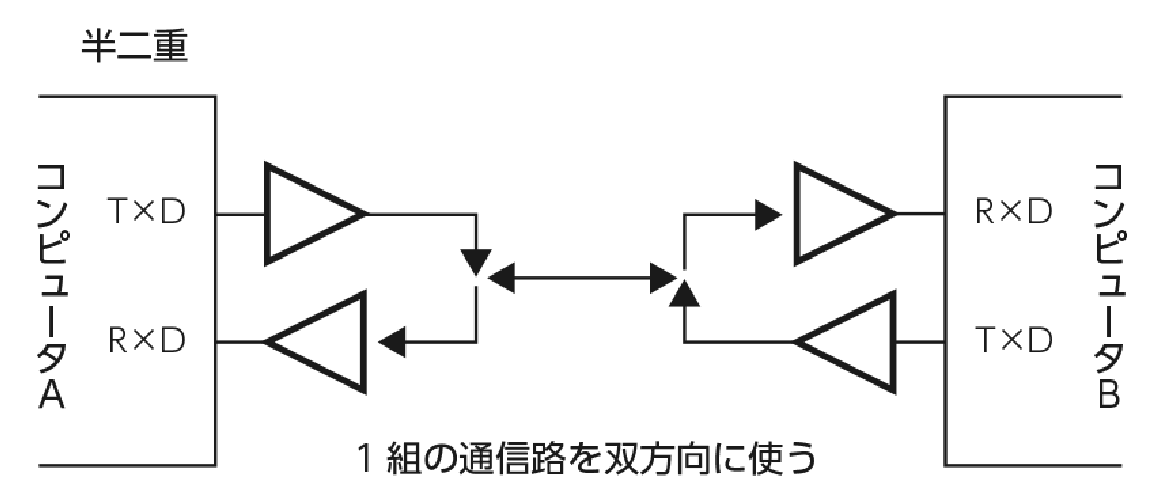
\includegraphics[width=0.7\linewidth,keepaspectratio]{fig/fig3_1.eps}
\caption{半二重通信の例:ThinkIT 新人エンジニアが知っておきたいネットワーク基礎知識 より引用}\label{fig3_1}
\end{figure}

電波や赤外線など、無線双方向通信は半二重通信によるものが多い(後に説明するFDDを用いた全二重通信のものもある\footnote{実用化されてはいないが、無線での(後に説明するFDDを用いない)全二重通信実現も研究されている。})。これは、同じ周波数の電波で信号を送る場合や同じ場所で赤外線通信を行う場合、双方が同時に送信したら混信・干渉してしまうためで、結果として通信路を1組しか用意できないということになる。先の糸電話とあまり変わらない例であるが、トランシーバーは一方が話していると来た方は話すことが出来ないため、半二重通信である。

半二重通信であっても、双方向の通信に十分な太さの回線で十分に短い時間で送受信を切り替えると、見かけ上は同時に送受信が行えるようになる。この方法を\textbf{時分割複信}\index{じぶんかつふくしん@時分割複信}(Time Division Duplex, \textbf{TDD} \index{TDD|see{時分割複信}})と呼ぶ。WiMAXなどがこの方式でサービスを提供している。

\subsection{全二重通信}
半二重通信とは異なり、そもそも線を2本用意するなどして双方が同時に送受信できるように通信を行えるようにした通信方式を\textbf{全二重通信}\index{ぜんにじゅうつうしん@全二重通信}(full duplex)と呼ぶ。先からあげている糸電話の例で言えば、糸電話を2組用意して、耳・口両方に対応するように当てることで同時会話を可能にしたものである。単方向2組であるため(図\ref{fig3_2})用意するべき設備自体が多くなるが、通信速度などの面でもっとも良い効果が得られる。
\begin{figure}[htb]
\centering
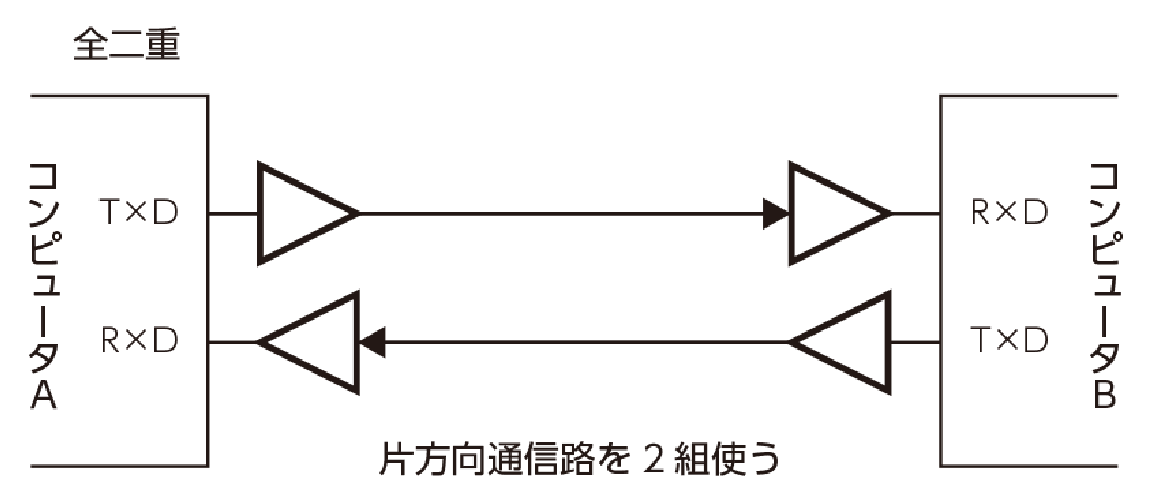
\includegraphics[width=0.7\linewidth,keepaspectratio]{fig/fig3_2.eps}
\caption{全二重通信の例:ThinkIT 新人エンジニアが知っておきたいネットワーク基礎知識 より引用}\label{fig3_2}
\end{figure}

現実世界の例では、固定電話が全二重通信を行っている。また、半二重通信の後に書いたが、LTEによる通信などは一つの伝送路で全二重通信を実現している。このLTEの例のように、一つの伝送路で全二重通信を実現する方法がある。先に挙げたTDDも見かけ上一つの伝送路で全二重通信を実現しているという意味ではその方法の一つである(厳密には半二重通信であるが)。

\subsubsection{周波数分割複信}
伝送を行うときにはある周波数を持った搬送波というものを用いることが多い(これについては後の章で詳しく見ていく)。このとき、異なる周波数の搬送波を用い、一方を上り方向・他方を下り方向と使い分けることで一つの伝送路で全二重通信を実現できる。この方法を\textbf{周波数分割複信}\index{しゅうはすうぶんかつふくしん@周波数分割複信}(Frequency Division Duplex, \textbf{FDD} \index{FDD|see{周波数分割複信}})と呼ぶ。先に挙げたLTEに限らず、無線通信で全二重通信を実現する場合は、TDDで見かけ上の全二重通信にするか、このFDDで全二重通信を実現する。有線では、ADSLが代表的な例と言える。ADSLでは多くを下りの周波数に割り当てて、通常ダウンロードの方が多い回線利用者に適合したサービスを提供している。

\subsubsection{エコーキャンセラ方式}
電話などの音声通信で同一の回線を使った場合、エコーがかかってしまうことがある。そこで、信号からエコーを除去して通信することで雑音を減らす手法が開発された。これを通常のデータ通信などに応用したものが\textbf{エコーキャンセラ方式}\index{えこーきゃんせらほうしき@エコーキャンセラ方式}である。信号を分けるハイブリッド回路などの仕組みを設け、送信信号と受信信号を分離する。そして送信信号のエコー分を除去して受信すれば、受信信号が得られる。欧米のISDN加入者線などで使われている方法である。また、複数周波数帯を用いた通信において、周波数の僅かな重なり(スペクトルオーバーラップ)を除去する用途などにも用いられている。

\section*{演習問題}
\begin{problems}
\item マイクには、ある方向・角度からでないと声が入りづらくなっている指向性マイクと、全方向からの声が等しく入る無指向性マイクがある。これを適切に使い分けることで雑音を減らすことができるが、それぞれどのような場面で使うのが適切か例示せよ。

\item レンタルサーバにおいては、稼働率99.9\%などと喧伝している業者もあり、これが達成されない場合は一部返金対応などが行われるなど、宣伝の材料としても用いられている。稼働率を基準にサービスを考える場合は、どの程度の時間に対応するか計算し、許容される停止時間を検討して決める必要がある。
\begin{enumerate}
\item 具体的に稼働率99\%,99.9\%,99.99\%の各レンタルサーバの年間停止時間を計算してみよ。
\item 年間の停止可能秒数が入力されるとき、期待される稼働率を出力するプログラムを作成せよ。
\end{enumerate}

\item 次の各ケーブルによる伝送について、半二重通信か全二重通信かを調べてみよ。
\begin{enumerate}
\item USB2.0ケーブル
\item USB3.0ケーブル
\item UTPケーブル(現在一般に使われるLANケーブル)
\item 同軸ケーブル
\end{enumerate}

\end{problems}
